%! Author = luciano
%! Date = 22/01/2020

% Preamble
\documentclass[11pt]{article}

% Packages
\usepackage{amsmath}
\usepackage[gobble=auto,
rerun=always
]{pythontex}
\usepackage{python}
\usepackage{cleveref}
\usepackage{enumerate}
\usepackage[utf8]{inputenc}
\usepackage[english]{babel}

\usepackage[ruled,linesnumbered,lined,boxed,commentsnumbered]{algorithm2e}
\SetStartEndCondition{ }{}{}%
\SetKwProg{Fn}{def}{\string:}{}
\SetKwInOut{Input}{Input}\SetKwInOut{Output}{Output}
\SetKwFunction{Range}{range}%%
\SetKwFunction{Len}{len}%%
\SetKwFunction{Statistic}{stat\_function}
\SetKwFunction{FnBoots}{bootstrap}
\SetKwFunction{FnBootsNP}{bootstrap\_np}
\SetKwArray{Data}{data}
\SetKwArray{Samples}{array\_of\_samples}
\SetKwArray{Sample}{sample$_{b}$}
\SetKwArray{Results}{result\_array}
\SetKw{KwTo}{in}\SetKwFor{For}{for}{\string:}{} \SetKwIF{If}{ElseIf}{Else}{if}{:}{elif}{else:}{} \SetKwFor{While}{while}{:}{fintq}
\newcommand{\forcond}{$b=0$ \KwTo $B$}
\renewcommand{\forcond}{$b$ \KwTo\Range{$B$}} \AlgoDontDisplayBlockMarkers\SetAlgoNoEnd\SetAlgoNoLine%

\usepackage[
backend=biber,
style=authoryear
]{biblatex}
\usepackage{graphicx}
\usepackage{float}

\addbibresource{References.bib}

% Document
\begin{document}

\section{Bootstrapping Functions}\label{sec:bootstrapping-functions}

\subsection{Basic Algorithm}\label{subsec:basic-algorithm}

According to \cite{LW04} we can define $T_n = g(X_1, \dots, X_n)$ as an statistic that depends on the data, and apply
bootstrapping for estimating the standard error and confidence intervals of $T_n$ for statistical inference. First,
\cite{LW04} proves that by using the law of large numbers, and assuming that we draw an IID sample of $Y_1, \dots, Y_B$,
we can conclude that as $B \rightarrow \infty$

\begin{align}
    \bar{Y} \overset{p}{\to} E(Y)
\end{align}
\begin{align}
    \frac{1}{B} \sum_{j=1}^{B}{(Y_j - \bar{Y})^{2}} \overset{p}{\to} V(Y)
\end{align}

Therefore, we can use the sample mean and the sample variance as an approximation for the population mean and variance.
Following the procedures stated by \cite{LW04}, we first assume that the data obtained initially follows a distribution
$\hat{F}_n$, from where we can take samples $X_{1}^{*}, \dots, X_{n}^{*}$ and compute $T_{n}^{*} = g(X_{1}^{*}, \dots, X_{n}^{*})$
$B$ times. From this step we will get a vector of $T_{n,1}^{*}, \dots, T_{n,B}^{*}$, from where we can compute the variance
(\cite{LW04}):

\begin{align}
v_{boot} = \frac{1}{B}\sum_{b=1}^{B}{\left( T_{n,b}^{*} - \frac{1}{B} \sum_{r=1}^{B}{T_{n,r}^{*}} \right)^2}
\end{align}

The standard error of the statistic $T_n$ is the square root of the variance, $SE = \sqrt{v_{boot}}$. Although there are
several methods to estimate the confidence interval of the statistics, we are going to use the percentiles of the statistic's
distribution. Consequently, the interval is defined as $C_n = \left(T_{\alpha/2}^{*},T_{1 - \alpha/2}^{*}\right)$.

\medskip

The previous can be resumed in Algorithm \ref{alg:AB} shows the steps followed more generally. One can observe that it divides the process
into three main parts: the first part generates $B$ samples, of $n_b$ size, from the original data using replacement,
the second part estimates the statistic $T_{n}$ for each $b$ sample, and, finally, the algorithm estimates the standard error and the
confidence interval. The sampling phase is a loop of size $B$ that applies a sampling function\footnotemark, therefore we can assume that
the time complexity of this process should be linear: $O(n)$, where $n$ is equal to $B$. (Analysis based on \cite{AL09})
Similarly, the second phase, is a process that estimates the statistic for each sample $b$, which should be bounded by
the same time complexity as the first phase if the statistic is simple enough, $O(n)$.
Finally, the last step estimates the variance and the confidence interval, which, assuming as given steps without
their own time complexity, have a constant time complexity $O(1)$. Under these assumptions, we can conclude that we expect
for the algorithm to have a linear time complexity $O(n)$, where the slope is determined by the number of samples taken from the
original data and the improvements made by using tools like parallel computing or optimized functions.

\footnotetext{We are assuming that the sampling function has a linear time complexity, since it can be understood as a
loop that generates a random number, under some specific conditions, to select an index of the input.}

\medskip

\begin{algorithm}[H]
    \KwData{A sample of a random variable $X$}
    \KwResult{A standard error and confidence interval}
    \tcc{Sampling phase}
    \For{\forcond}{
        select $X_{1, b}^{*}, \dots, X_{n,b}^{*}$ elements of the original data using replacement\; }
    \tcc{Estimation phase}
    \For{\forcond}{
        estimate $T_{n,b}^{*}$ for the $b$ sample\;}
    \tcc{Results phase}
    estimate the square root of the variance of the statistics and the confidence interval
\caption{Bootstrapping}\label{alg:AB}
\end{algorithm}

\medskip
\medskip

This algorithm could be translated into the following Python code following the steps mentioned by \cite{LW04}. As an
example, we are going to assume that the original data comes from a normal distribution with $\mu = 5$ and $\sigma^2 = 1$
and we want to estimate the standard error and the confidence interval for the statistic, which in this case is the mean.


\begin{pyblock}
import numpy as np
from scipy.stats import norm
# Assume we have a random sample from a normal distribution
np.random.seed(11)
sample_normal = np.random.normal(5, 1, 10000)

# 1. Generate 1000 random samples with replacement
samples = np.array([np.random.choice(sample_normal,
                    size=100, replace=True) for _ in range(1000)])

# 2. Estimate the mean (statistic) for each random sample
mean_dist = np.array([np.mean(x) for x in samples])

# 3. Estimate the standard error and the confidence interval
se_mean = np.sqrt(np.var(mean_dist))
confint_mean = np.percentile(mean_dist, [2.5, 97.5])
print("Standard Error: ",  round(se_mean, 3),
        "\n95% Confidence Interval: ", round(confint_mean[0], 3),
        " - ", round(confint_mean[1], 3))
\end{pyblock}

\printpythontex[verbatim]

\medskip

The main results from the algorithm are the standard error and the confidence interval of the statistic (i.e. mean), additionally
we can observe the behavior of the bootstrap results in a histogram which, in the case of estimating the mean, illustrates the central
limit theorem. Figure \ref{fig:BootsExample} shows the histogram of the bootstrap samples for the mean with the density kernel of
the observed data (blue line), and the normal distribution (black line). Theory tells us that (\cite{LW04}), by the central limit theorem,
the distribution of the sample mean converges in distribution to a $N(\mu, \sigma^2)$. With this, one can establish
probability statements about the mean of the random variable $X$.


\begin{pycode}
from pylab import *
rc('font', family='serif')
rc('font', size=10.0)
rc('legend', fontsize=10.0)
rc('font', weight='normal')
import numpy as np
from scipy.stats import norm
import seaborn as sns
# Assume we have a random sample from a normal distribution
np.random.seed(11)
sample_normal = np.random.normal(5, 1, 10000)
# 1. Generate 1000 random samples with replacement
samples = np.array([np.random.choice(sample_normal,
                    size=100, replace=True) for _ in range(1000)])
# 2. Estimate the mean (statistic) for each random sample
mean_dist = np.array([np.mean(x) for x in samples])
# 3. Estimate the standard error and the confidence interval
se_mean = np.sqrt(np.var(mean_dist))
confint_mean = np.percentile(mean_dist, [2.5, 97.5])
figure(figsize=(4, 2.5))
axvspan(confint_mean[0], confint_mean[1], facecolor='g', alpha=0.4, ymin=0, ymax=0.05)
sns.distplot(mean_dist, axlabel='Histogram of Bootstrap Samples', fit = norm)
axvline(x = 5, linewidth=2, color='r', alpha = 0.5)
axvline(x=5 - se_mean, linewidth=2, color='orange', ymin=0, ymax=0.1, alpha = 0.8)
axvline(x=5 + se_mean, linewidth=2, color='orange', ymin=0, ymax=0.1, alpha = 0.8)
xlabel('Statistic values')
ylabel('Frequency')
savefig('mean_dist.pdf', transparent=True)
\end{pycode}

\begin{figure}[H]
    \begin{center}
        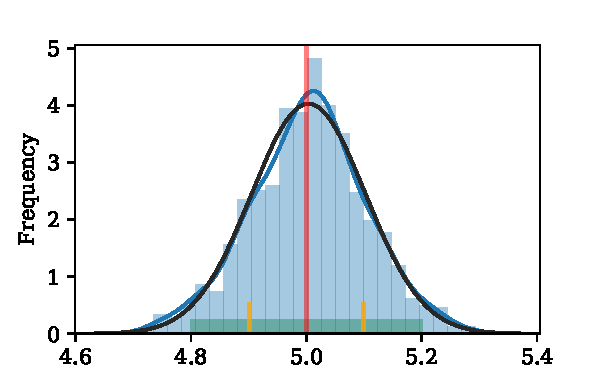
\includegraphics{mean_dist.pdf}
    \end{center}
    \caption{Histogram and density plot of the bootstrap samples. \textit{Note}:
    confidence interval in green area, standard errors in orange and normal distribution in black}\label{fig:BootsExample}
\end{figure}

\medskip

The algorithm implemented shows the expected results with respect to the statistical objectives, however, the main focus
of this study is to analyze the performance of bootstrapping when using parallel computing. The next sections will divide
the problem between a non-parallel version (i.e. serial) and a parallel implementation of the bootstrapping algorithm.

\subsection{Serial Algorithms}\label{subsec:serial-algorithms}

The serial version of bootstrapping replicates the steps followed by the Algorithm \ref{alg:AB} with only one processor
of the computer. At this point, to construct a function that executes the algorithm, a main aspect is the generation
of random numbers for the sampling phase. We decided to use two types of generators to understand how the performance of
the algorithm can change based on specific changes on each step. The two options are: the \texttt{random} package
of python core libraries (Algorithm \ref{alg:AB2}) and \texttt{Numpy} package (Algorithm \ref{alg:AB3}). It is noteworthy
that the first implementation uses a nested loop (line \ref{NestedLoop}), incrementing the time complexity to a polynomial
form $O(mn)$, where $m$ is the size of the samples. Therefore, we can expect that the time complexity of the function
that uses \texttt{numpy} is bounded by the function without \texttt{numpy}.

\medskip

\begin{algorithm}[H]
    \Input{A sample of a random variable $X$}
    \Output{A object with the standard error and confidence interval}
    \BlankLine
    \Fn{\FnBoots{input, statistic function, number of samples, size of sample}}{
    \tcc{Sampling phase}
    \For{\forcond}{\label{ForSerial1}
        \For{$j$ \KwTo \Range{size of samples}}{\label{NestedLoop}
        \tcp{Using \texttt{random.randint} module}
        \textit{index} = create a random integer $\in$ [0, \Len{\Data{n}} - 1]\;
        \Sample{$j$} = \Data{\textit{index}}\;}
    }

    \tcc{Estimation phase}
    \For{\forcond}{
        \Results{b} = \Statistic{\Samples{b}}\;}
    \tcc{Results phase}
    estimate the square root of the variance of the statistics and the confidence interval\;
    }
\caption{Serial Bootstrapping without \texttt{Numpy}}\label{alg:AB2}
\end{algorithm}

\medskip

On the other hand, on Algorithm \ref{alg:AB3} we replicated the Algorithm \ref{alg:AB2} using the \texttt{numpy} package
to generate the samples from the original data.
Since \texttt{numpy} is a scientific package made to optimize processes like bootstrapping, we
expect a improvement in terms of performance when both functions are compared. The Algorithm \ref{alg:AB3} enumerates the
steps taken by the function to execute the bootstrapping. The main difference with the previous function resides in the
\texttt{for loop} at line \ref{ForSerialNP1} in Algorithm \ref{alg:AB3}, since we avoided the introduction of an additional
\texttt{for loop}. Therefore, we could assume that the time complexity of this algorithm is $O(n)$, since it just performs
the sample and estimation in one \texttt{for loop}.

\begin{algorithm}[H]
    \Input{A sample of a random variable $X$}
    \Output{A object with the standard error and confidence interval}
    \BlankLine
    \Fn{\FnBootsNP{input, statistic function, number of samples, size of sample}}{
    \tcc{Sampling phase and Estimation phase}
    \For{\forcond}{\label{ForSerialNP1}
        \tcp{Using \texttt{numpy.random.choice}}
        \Samples{b} = create a random sample of determined size from \Data \;
        \Results{b} = \Statistic{\Samples{b}}\;}

    \tcc{Results phase}
    estimate the square root of the variance of the statistics and the confidence interval\;
    }
\caption{Serial Bootstrapping with \texttt{Numpy}}\label{alg:AB3}
\end{algorithm}

\medskip

To further analyze the performance of the algorithms, we first implemented a test to generate a range of $B$ samples, since
this is the main argument of the bootstrap function that could affect the performance of the functions. The range of the test
has a minimum of $B = 1,000$ samples up to $B = 1,000,000$ samples by steps of $10,000$. For each implementation of the
algorithm, we time the performance using the \texttt{timeit} module of Python libraries, which returns an average time for
each run. The results are presented in the Figure \ref{fig:SerialTest}, where the straight blue line is the function
without \texttt{numpy}, and the dashed line is the function in Algorithm \ref{alg:AB3}. In average, the function with Numpy
is 8.64 times faster than the function without this package, confirming our hypothesis of the difference of the time complexity
between both algorithms.

\medskip

\begin{pycode}
from pylab import *
rc('font', family='serif')
rc('font', size=8.0)
rc('legend', fontsize=8.0)
rc('font', weight='normal')
import numpy as np
import pandas as pd
import matplotlib.ticker as ticker
from scipy.stats import norm
import seaborn as sns
data = pd.read_pickle('data/NoNPvsNPv2.pkl')
data_wo = data.loc[:, ['Serial', 'SerialNP']]
data_wo = data_wo.rename(columns={"Serial": "Without Numpy", "SerialNP": "With Numpy"})
clf()
figure(figsize=(5, 4.5))
sns.set(style='darkgrid', palette='Paired')
p = sns.lineplot(data=data_wo, dashes=[(None, None), (2, 2)])
p.xaxis.set_major_formatter(ticker.FuncFormatter(lambda x, pos: '{:,.0f}'.format(x)))
p.set(xlabel = 'Size (number of samples)', ylabel = 'Running Time', title = 'Serial Implementation')
savefig('serial_test.pdf')
\end{pycode}

\begin{figure}[H]
    \begin{center}
        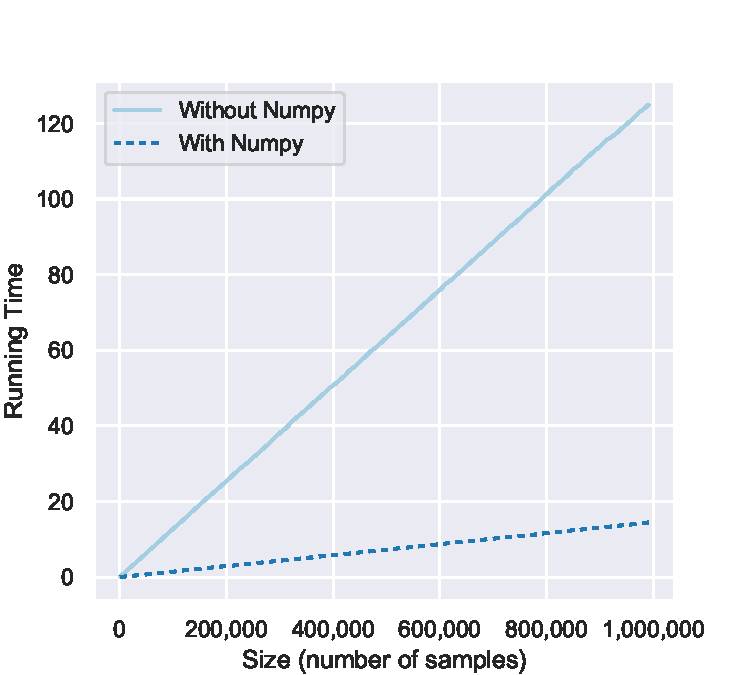
\includegraphics{serial_test.pdf}
    \end{center}
    \caption{Bootstrapping Test for Serial Functions}\label{fig:SerialTest}
\end{figure}

\subsection{Parallel Algorithms}\label{subsec:parallel-algorithms}



\printbibliography

\end{document}